\documentclass[tikz,border=0pt]{standalone}
\usepackage[T1]{fontenc}
\usepackage{lmodern,amsmath,amssymb}
\usetikzlibrary{arrows.meta,calc,positioning}
\definecolor{blue}{HTML}{0072B2}
\definecolor{orange}{HTML}{D55E00}
\definecolor{green}{HTML}{009E73}
\definecolor{purple}{HTML}{8C5694}
\definecolor{ink}{HTML}{25313B}
\renewcommand{\familydefault}{\sfdefault}
\begin{document}
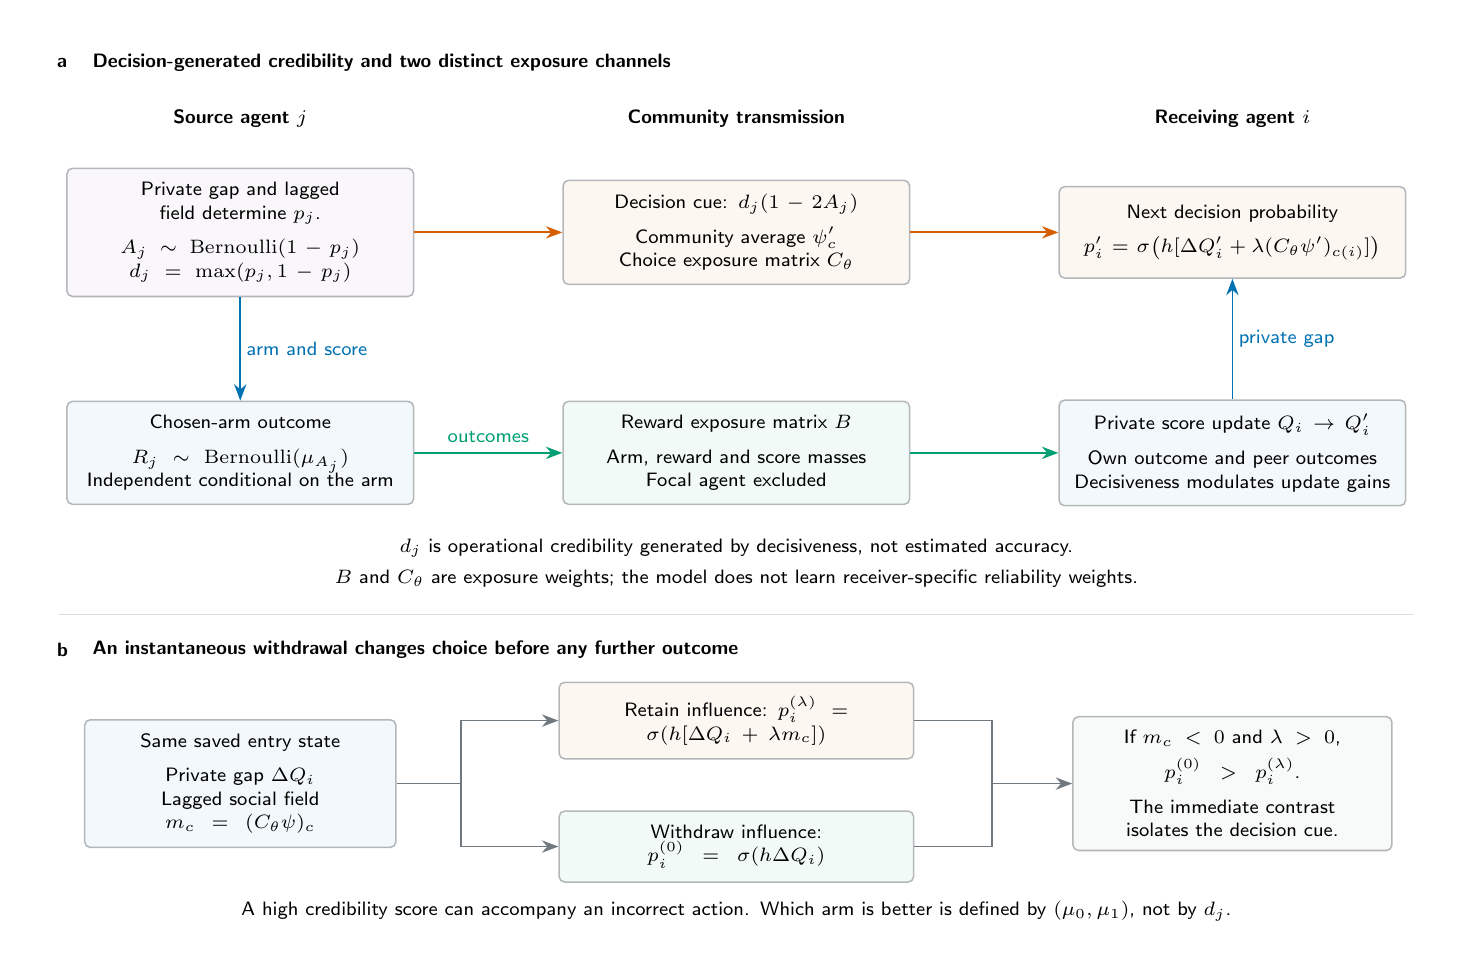
\begin{tikzpicture}[x=1cm,y=1cm,font=\sffamily\fontsize{7}{8.5}\selectfont,>=Stealth,
 box/.style={draw=ink!35,fill=white,rounded corners=2pt,align=center,text width=4.05cm,minimum height=1.16cm,inner sep=5pt,line width=.55pt},
 arr/.style={->,line width=.65pt,draw=ink!65},
 head/.style={font=\sffamily\fontsize{7}{8.5}\selectfont\bfseries,anchor=west},
 letter/.style={font=\sffamily\fontsize{7}{8.5}\selectfont\bfseries,anchor=west}]
 \path[use as bounding box] (0,0) rectangle (18,11.5);
 \node[letter] at (.25,11.05) {a};
 \node[head] at (.7,11.05) {Decision-generated credibility and two distinct exposure channels};
 \node[head,anchor=center] at (2.7,10.35) {Source agent $j$};
 \node[head,anchor=center] at (9,10.35) {Community transmission};
 \node[head,anchor=center] at (15.3,10.35) {Receiving agent $i$};
 \node[box,fill=purple!5] (source) at (2.7,8.9) {Private gap and lagged field determine $p_j$.\\[4pt]$A_j\sim\mathrm{Bernoulli}(1-p_j)$\\$d_j=\max(p_j,1-p_j)$};
 \node[box,fill=orange!5] (cue) at (9,8.9) {Decision cue: $d_j(1-2A_j)$\\[4pt]Community average $\psi_c'$\\Choice exposure matrix $C_\theta$};
 \node[box,fill=orange!5] (decision) at (15.3,8.9) {Next decision probability\\[4pt]$p_i'=\sigma\!\left(h[\Delta Q_i'+\lambda(C_\theta\psi')_{c(i)}]\right)$};
 \node[box,fill=blue!5] (reward) at (2.7,6.1) {Chosen-arm outcome\\[4pt]$R_j\sim\mathrm{Bernoulli}(\mu_{A_j})$\\Independent conditional on the arm};
 \node[box,fill=green!5] (peer) at (9,6.1) {Reward exposure matrix $B$\\[4pt]Arm, reward and score masses\\Focal agent excluded};
 \node[box,fill=blue!5] (private) at (15.3,6.1) {Private score update $Q_i\to Q_i'$\\[4pt]Own outcome and peer outcomes\\Decisiveness modulates update gains};
 \draw[arr,orange] (source.east)--(cue.west);
 \draw[arr,orange] (cue.east)--(decision.west);
 \draw[arr,blue] (source.south)--node[right,fill=white,inner sep=2pt] {arm and score} (reward.north);
 \draw[arr,green] (reward.east)--node[above] {outcomes} (peer.west);
 \draw[arr,green] (peer.east)--(private.west);
 \draw[arr,blue] (private.north)--node[right,fill=white,inner sep=2pt] {private gap} (decision.south);
 \node[align=center,text width=16.6cm] at (9,4.7) {$d_j$ is operational credibility generated by decisiveness, not estimated accuracy.\\[3pt]$B$ and $C_\theta$ are exposure weights; the model does not learn receiver-specific reliability weights.};
 \draw[ink!16,line width=.5pt] (.4,4.05)--(17.6,4.05);
 \node[letter] at (.25,3.6) {b};
 \node[head] at (.7,3.6) {An instantaneous withdrawal changes choice before any further outcome};
 \node[box,fill=blue!5,text width=3.6cm] (state) at (2.7,1.9) {Same saved entry state\\[4pt]Private gap $\Delta Q_i$\\Lagged social field $m_c=(C_\theta\psi)_c$};
 \node[box,fill=orange!5,text width=4.15cm,minimum height=.8cm] (retain) at (9,2.7) {Retain influence: $p_i^{(\lambda)}=\sigma(h[\Delta Q_i+\lambda m_c])$};
 \node[box,fill=green!5,text width=4.15cm,minimum height=.8cm] (remove) at (9,1.1) {Withdraw influence: $p_i^{(0)}=\sigma(h\Delta Q_i)$};
 \node[box,fill=ink!3,text width=3.7cm] (effect) at (15.3,1.9) {If $m_c<0$ and $\lambda>0$,\\[4pt]$p_i^{(0)}>p_i^{(\lambda)}$.\\[4pt]The immediate contrast\\isolates the decision cue.};
 \draw[arr] (state.east)--(5.5,1.9)|-(retain.west);
 \draw[arr] (5.5,1.9)|-(remove.west);
 \draw[draw=ink!65,line width=.65pt] (retain.east)--(12.25,2.7)--(12.25,1.1)--(remove.east);
 \draw[arr] (12.25,1.9)--(effect.west);
 \node[align=center,text width=16.6cm] at (9,.28) {A high credibility score can accompany an incorrect action. Which arm is better is defined by $(\mu_0,\mu_1)$, not by $d_j$.};
\end{tikzpicture}
\end{document}
